\chapter{Related Work}
As with many fields in robotics, Human Robot Interaction (HRI) has seen a lot of developement in the last twenty years. Research has come from teleoperated assistive robots tho dynamically and independently collaborating robots. This advancement is expressed by the newly joined terms in literature to differentiate between types of interaction and level of autonomy for the robot.

\chapter{Mobile Manipulator}
We conduct or research on a mobile manipulator, lovingly called the \emph{Thing}. It is composed of four main components, on which we elaborate in detail in this chapter. The first is the Ridgeback, a omnidirectional robot platform , followed by the UR10, a six degrees of freedom (DOF) robot arm with a three finger gripper as it's end effector. A force torque sensor is embedded in the wrist of the gripper. The whole manipulator is an out of the box system assembled by Clearpath, which collaborates with Universal Robots and Robotiq and mounts the parts on the platform in house.

\section{Ridgeback}

\begin{figure}
   \centering
   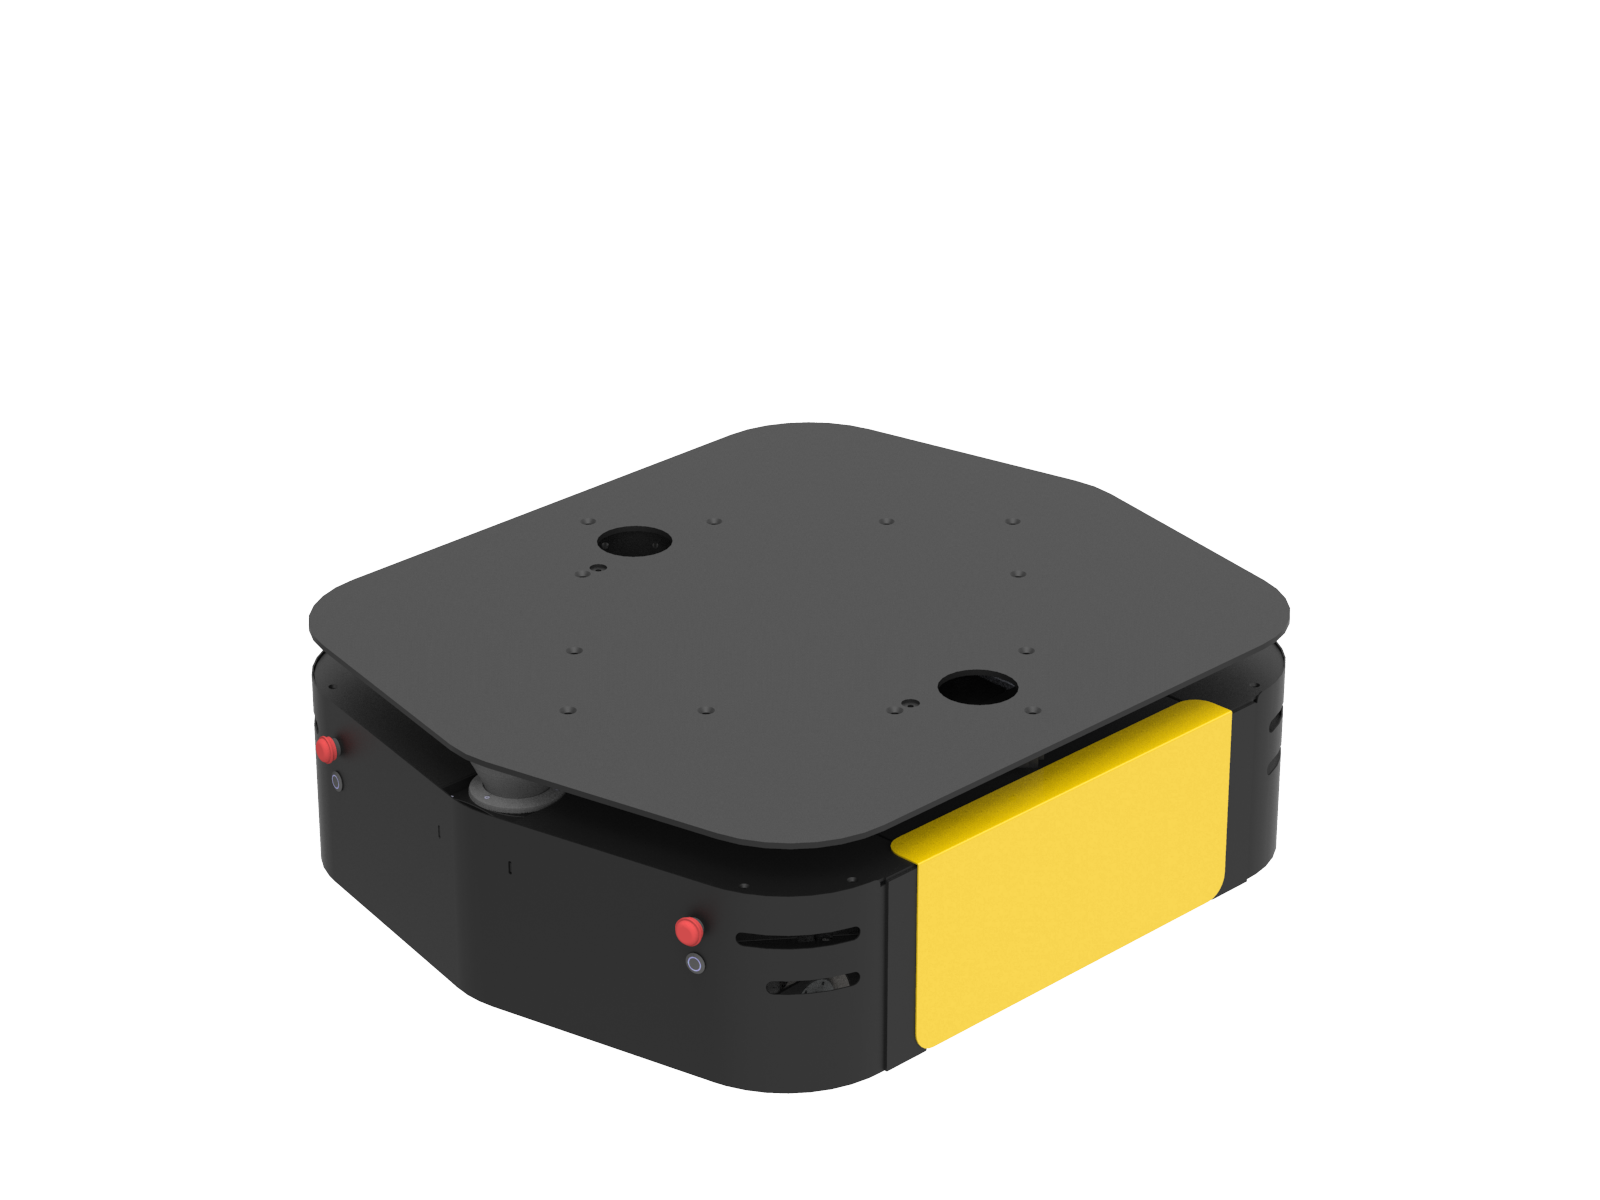
\includegraphics[width=0.75\textwidth]{images/ridgeback.png}
   \caption{Clearpath Ridgeback}
   \label{pics:ridgeback}
\end{figure}

\begin{table}[h]
\begin{center}
 \caption{Clearpath Ridgeback Specifications}\vspace{1ex}
 \label{tab:ridgeback}
 \begin{tabular}{ll}
 \hline
 Length & \unit[960]{mm}\\
 Width & \unit[793]{mm}\\
 Height & \unit[296]{mm}\\
 Weight & \unit[135]{kg}\\
 Maximum payload & \unit[100]{kg}\\
 Maximum velocity & \unitfrac[1.1]{m}{s}\\
 Average power consumption & \unit[800]{W}\\
 \hline
 \end{tabular}
\end{center}
\end{table}

The ridgeback is an omnidirectional robot platform designed by Clearpath for indoor movement and payload carrying tasks, such as autonomous warehousing for example. It is a fully integrated system with sensors, actuation and control and features a native ROS interface. Onboard sensors consist of an IMU and a front facing Hokuyo laser range finder (LIDAR) and a Kinect2 camera and wheel odometry. Optionally, a second, rear facing LIDAR can be mounted for full \unit[360]{\textdegree} coverage.The broad range of sensors, it's flexibility and low drift in odometry makes the Ridgeback a suitable and popular platform for research in controlled indoor environments.

Additionally, the Ridgeback houses the onboard computer that runs the low-level drivers of all the elements of the manipulator. On top thereof, there is a high-level driver that ensures accord and offers a ROS interface for the user to connect to.

\section{Universal Robot 10}

\begin{figure}
   \centering
   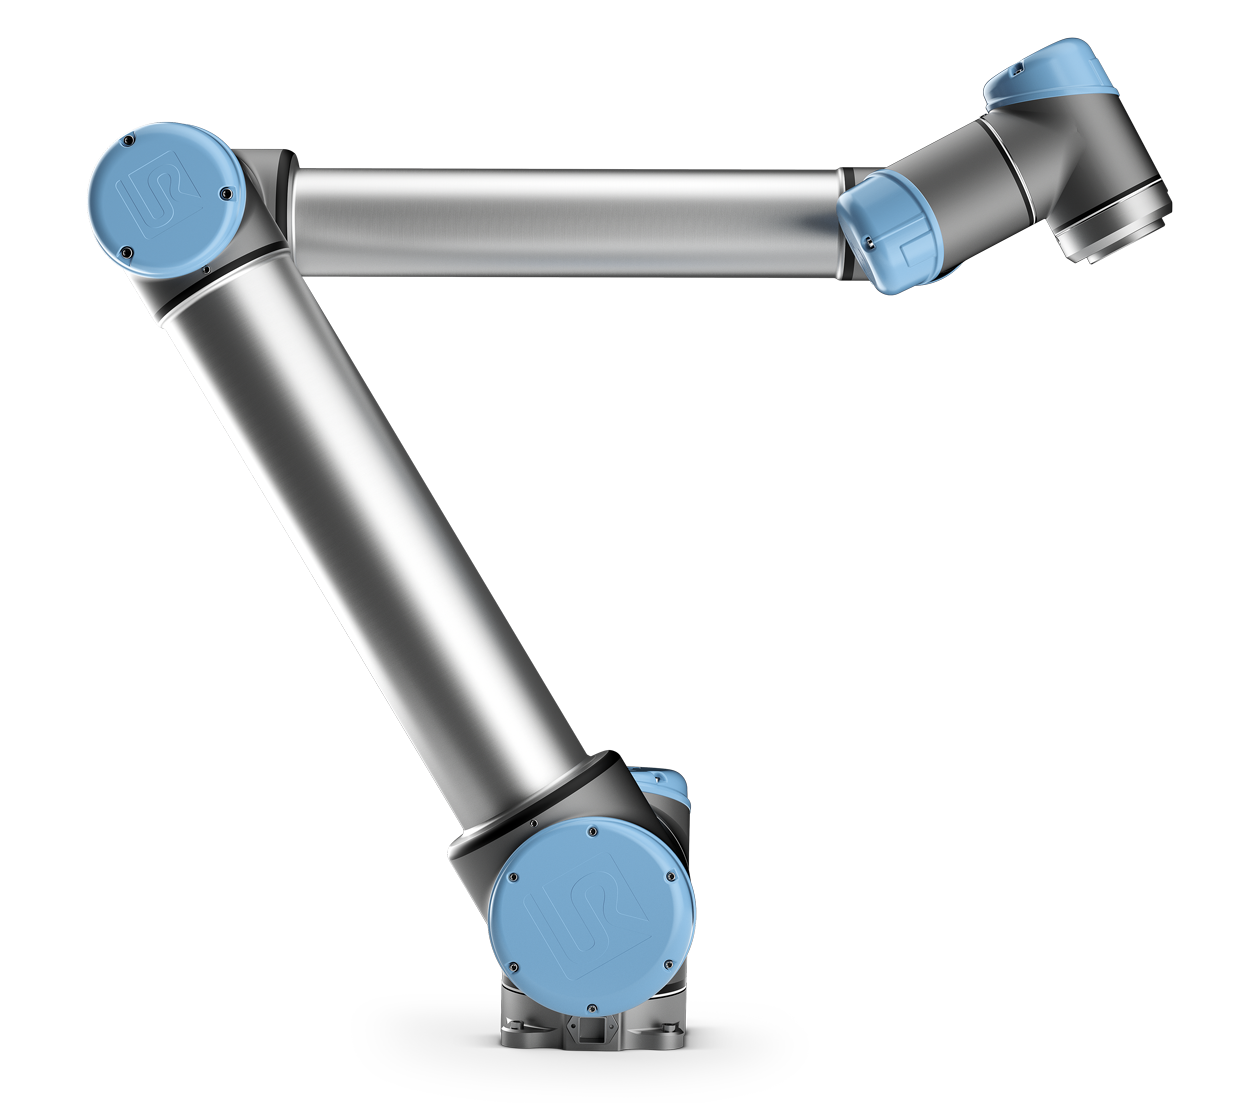
\includegraphics[width=0.75\textwidth]{images/ur10.png}
   \caption{Universal Robot 10}
   \label{pics:ur10}
\end{figure}

The UR10 is an collaborative industrial robot arm by Universal Robots. It has six rotary joints with gives it six DOF and can support payloads up to \unit[10]{kg}. Together with it's little brother the UR5, it is widely regarded as the standard manipulator within robotics research. Hence, extensive platform and software integration resources are available and ROS is supported out of the box.

\begin{table}[h]
\begin{center}
 \caption{Universal Robot 10 Specifications}\vspace{1ex}
 \label{tab:ur10}
 \begin{tabular}{ll}
 \hline
 Reach & \unit[1300]{mm} \\
 Weight & \unit[1.5]{kg}\\
 Repeatability & \unit[0.1]{mm} \\
 Maximum payload & \unit[10]{kg}\\
 Maximum tool velocity & \unitfrac[1]{m}{s}\\
 Degrees of freedom & 6 rotating joints \\
 Average power consumption & \unit[]{W}\\
 \hline
 \end{tabular}
\end{center}
\end{table}

\section{Gripper}

\begin{figure}
   \centering
   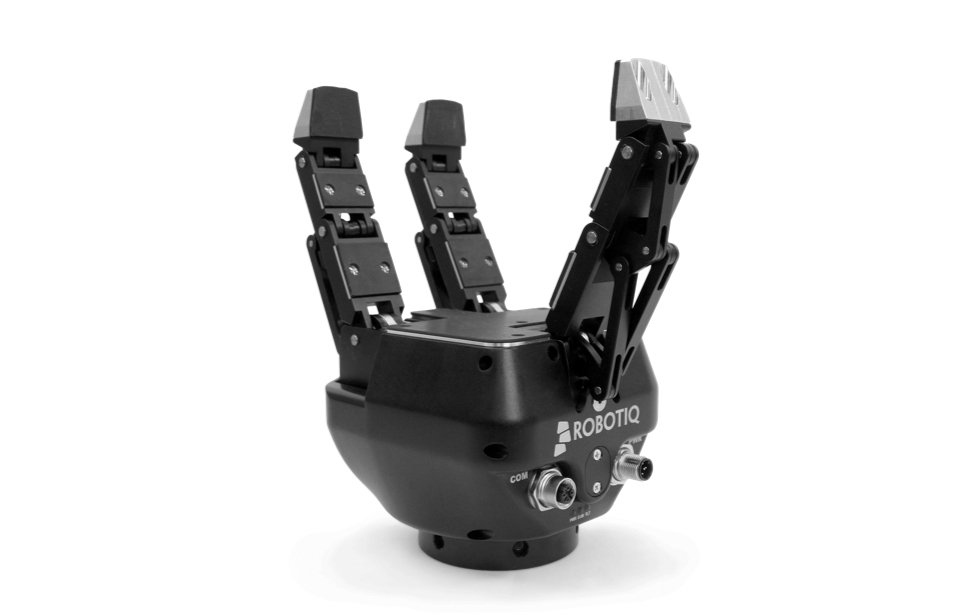
\includegraphics[width=0.75\textwidth]{images/robotiq_gripper.jpg}
   \caption{Robotiq 3-Finger Adaptive Robot Gripper}
   \label{pics:robotiq_gripper}
\end{figure}

\begin{table}[h]
\begin{center}
 \caption{Robotiq 3-Finger Adaptive Robot Gripper Specifications}\vspace{1ex}
 \label{tab:robotiq_gripper}
 \begin{tabular}{ll}
 \hline
 Weight & \unit[2.3]{kg}\\
 Repeatability & \unit[0.1]{mm} \\
 Maximum payload (encompassing grip) & \unit[10]{kg}\\
 Gripper opening & \unit[0 to 155]{mm} \\
 Object diameter for encompassing & \unit[20 to 155]{mm}\\
 Grip force & \unit[30 to 70]{N} \\
 Minimum power consumption & \unit[4.1]{W} \\
 Peak power (at maximum gripping force) & \unit[36]{W}\\
 \hline
 \end{tabular}
\end{center}
\end{table}

\section{Force-Torque Sensor}

\begin{figure}
   \centering
   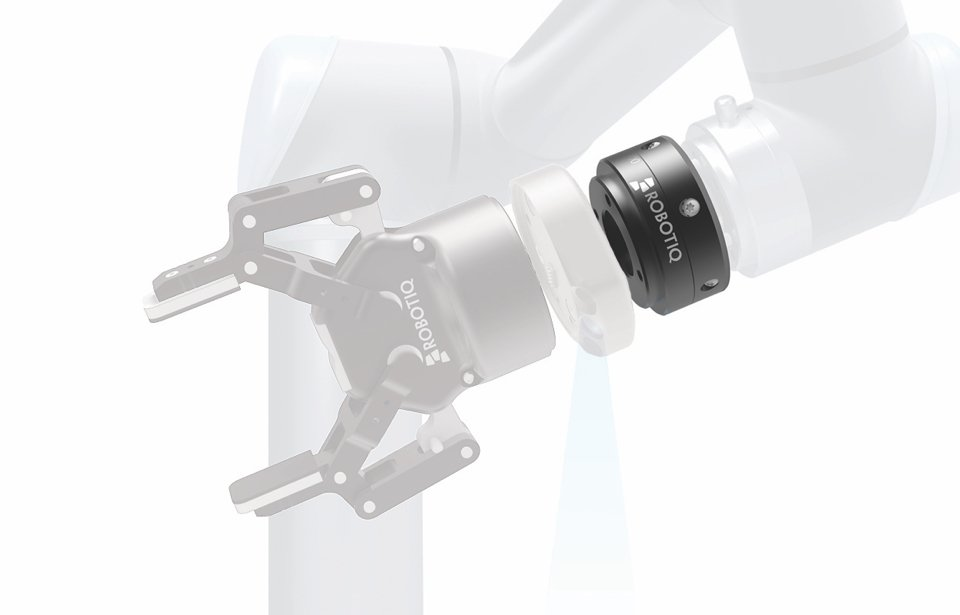
\includegraphics[width=0.75\textwidth]{images/robotiq_ft.jpg}
   \caption{Robotiq FT 300 Force Torque Sensor}
   \label{pics:robotiq_ft}
\end{figure}

\begin{savenotes}
\begin{table}[h]
\begin{center}
 \caption{Robotiq FT 300 Force Torque Sensor Specifications}\vspace{1ex}
 \label{tab:robotiq_ft}
 \begin{tabular}{ll}
 \hline
 \textbf{Measuring range} & \\
 Force $F_x, F_y, F_z$ & \unit[$\pm 300$]{N} \\
 Moment $M_x, M_y, M_z$ & \unit[$\pm 30$]{Nm} \\ \hline
 \textbf{Signal noise}\footnote{Signal noise is the standard deviation of the signal measured over a period of one second.} &\\
 Force $F_x, F_y, F_z$ & \unit[0.1]{N} / \unit[1]{N} \\
 Moment $M_x, M_y$ & \unit[0.05]{Nm} / \unit[0.02]{Nm} \\
 Moment $M_z$ & \unit[0.03]{Nm} / \unit[0.01]{Nm} \\ \hline
 Data output rate & \unit[100]{Hz} \\
 Weight & \unit[300]{g}\\
 \hline
 \end{tabular}
\end{center}
\end{table}
\end{savenotes}

\chapter{Thing Control Structure}

\chapter{Admittance Control}

\chapter{Obstacle Avoidance}
\section{Global Planner}
\section{Local Planner}

We use the Dynamic Window Approach (DWA) \citep{fox1997dynamic} for local collision avoidance. This well-known algorithm produces command velocities for a planar robot given vehicle dynamics and obstacle measurements. The basic assumption is that the robot moves instantaneously on circular arcs with a translational velocity $v$ and a rotational velocity $\omega$. Thus, the complexity is greatly simplified and calculations are be performed in the 2D velocity space $(v,\omega)$. Within this space, we compute three sets of velocity pairs,  subsequently called \emph{windows} for every iteration of the algorithm.

The \emph{obstacle window} $V_o$ are the measurements of any obstacles, e.g. taken by a range laser sensor and transformed from cartesian to $v,\omega$ space.

The \emph{static window} $V_s$ expresses the constraint velocities of the vehicle, i.e., absolute maximum and minimum velocity. As the name suggests, these parameters are usually static and do not need to be recalculated every step.

The \emph{dynamic window} $V_d$ are the vehicle dynamics, i.e., velocities that are physically feasible for the robot to reach within one timestep. It's size is defined by the maximal acceleration and the current velocity of the robot.

\begin{equation}
V_r = V_o \cap V_s \cap V_d
 	\label{eq:dwa_intersection}
\end{equation}

As Equation \cref{eq:dwa_intersection} shows, the intersection of these three sets gives us the resulting window $V_r$ of feasible velocity pairs, that guarantee no collision with an obstacle for the next step.

A cost function is then applied to find the $(v,\omega)$ pair, that maximizes the objective within $V_r$. Elements are heading, distance to goal and velocity terms.

\chapter{Results}

\chapter{Conclusions}

\chapter{Einige wichtige Hinweise zum Arbeiten mit \LaTeX\ }
\label{sec:latexumg}

Nachfolgend wird die Codierung einiger oft verwendeten Elemente
kurz beschrieben. Das Einbinden von Bildern ist in \LaTeX\ nicht
ganz unproblematisch und hängt auch stark vom verwendeten Compiler
ab. Typisches Format für Bilder in \LaTeX\ ist
EPS\footnote{Encapsulated Postscript} oder PDF\footnote{Portable Document Format}.


\section{Gliederungen}
\label{sec:gliederung}

Ein Text kann mit den Befehlen \texttt{\textbackslash
chapter\{.\}}, \texttt{\textbackslash section\{.\}},
\texttt{\textbackslash subsection\{.\}} und \texttt{\textbackslash
subsubsection\{.\}} gegliedert werden.


\section{Referenzen und Verweise}
\label{sec:refverw}

Literaturreferenzen werden mit dem Befehl \texttt{\textbackslash
citep\{.\}} und \texttt{\textbackslash
citet\{.\}} erzeugt. Beispiele: ein Buch \citep{Raibert1986LeggedRobotsThatBalance}, ein Buch und ein Journal Paper \citep{Raibert1986LeggedRobotsThatBalance,Vukobratovic2004ZeroMomentPoint}, ein Konferenz Paper mit Erwähnung des Autors: \citet{Pratt1995SEA}.

Zur Erzeugung von Fussnoten wird der Befehl \texttt{\textbackslash
footnote\{.\}} verwendet. Auch hier ein Beispiel\footnote{Bla
bla.}.

Querverweise im Text werden mit \texttt{\textbackslash label\{.\}}
verankert und mit \texttt{\textbackslash cref\{.\}} erzeugt.
Beispiel einer Referenz auf das zweite Kapitel:
\cref{sec:latexumg}.


\section{Aufzählungen}\label{sec:aufz}

Folgendes Beispiel einer Aufzählung ohne Numerierung,
\begin{itemize}
  \item Punkt 1
  \item Punkt 2
\end{itemize}
wurde erzeugt mit:
\begin{verbatim}
\begin{itemize}
  \item Punkt 1
  \item Punkt 2
\end{itemize}
\end{verbatim}

Folgendes Beispiel einer Aufzählung mit Numerierung,
\begin{enumerate}
  \item Punkt 1
  \item Punkt 2
\end{enumerate}
wurde erzeugt mit:
\begin{verbatim}
\begin{enumerate}
  \item Punkt 1
  \item Punkt 2
\end{enumerate}
\end{verbatim}

Folgendes Beispiel einer Auflistung,
\begin{description}
  \item[P1] Punkt 1
  \item[P2] Punkt 2
\end{description}
wurde erzeugt mit:
\begin{verbatim}
\begin{description}
  \item[P1] Punkt 1
  \item[P2] Punkt 2
\end{description}
\end{verbatim}


\section{Erstellen einer Tabelle}\label{sec:tabellen}

Ein Beispiel einer Tabelle:
\begin{table}[h]
\begin{center}
 \caption{Daten der Fahrzyklen ECE, EUDC, NEFZ.}\vspace{1ex}
 \label{tab:tabnefz}
 \begin{tabular}{ll|ccc}
 \hline
 Kennzahl & Einheit & ECE & EUDC & NEFZ \\ \hline \hline
 Dauer & s & 780 & 400 & 1180 \\
 Distanz & km & 4.052 & 6.955 & 11.007 \\
 Durchschnittsgeschwindigkeit & km/h & 18.7 &  62.6 & 33.6 \\
 Leerlaufanteil & \% & 36 & 10 & 27 \\
 \hline
 \end{tabular}
\end{center}
\end{table}

Die Tabelle wurde erzeugt mit:
\begin{verbatim}
\begin{table}[h]
\begin{center}
 \caption{Daten der Fahrzyklen ECE, EUDC, NEFZ.}\vspace{1ex}
 \label{tab:tabnefz}
 \begin{tabular}{ll|ccc}
 \hline
 Kennzahl & Einheit & ECE & EUDC & NEFZ \\ \hline \hline
 Dauer & s & 780 & 400 & 1180 \\
 Distanz & km & 4.052 & 6.955 & 11.007 \\
 Durchschnittsgeschwindigkeit & km/h & 18.7 &  62.6 & 33.6 \\
 Leerlaufanteil & \% & 36 & 10 & 27 \\
 \hline
 \end{tabular}
\end{center}
\end{table}
\end{verbatim}


\section{Einbinden einer Grafik}\label{sec:epsgraph}

Das Einbinden von Graphiken kann wie folgt bewerkstelligt werden:
\begin{verbatim}
\begin{figure}
   \centering
   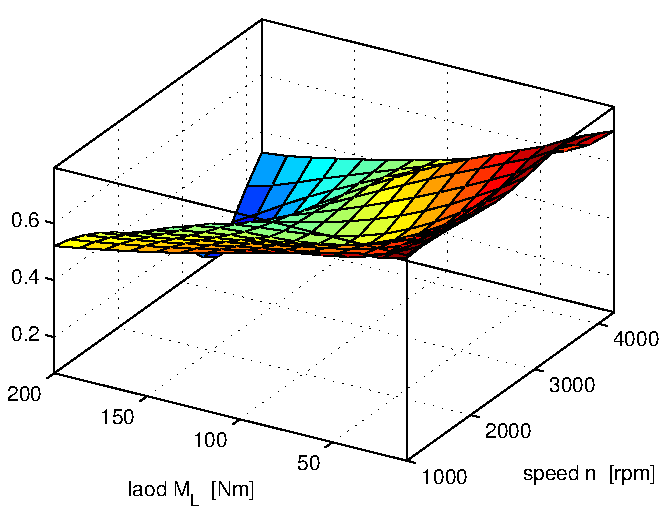
\includegraphics[width=0.75\textwidth]{images/k_surf.pdf}
   \caption{Ein Bild.}
   \label{fig:k_surf}
\end{figure}
\end{verbatim}

\begin{figure}
   \centering
   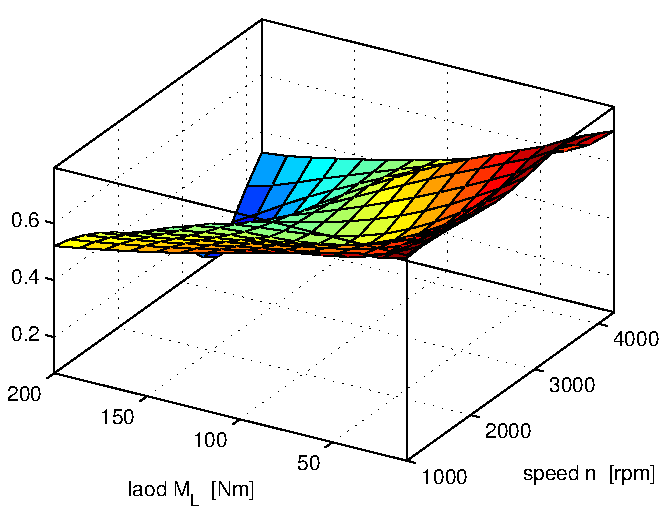
\includegraphics[width=0.75\textwidth]{images/k_surf.pdf}
   \caption{Ein Bild}
   \label{pics:k_surf}
\end{figure}

oder bei zwei Bildern nebeneinander mit:
\begin{verbatim}
\begin{figure}
  \begin{minipage}[t]{0.48\textwidth}
    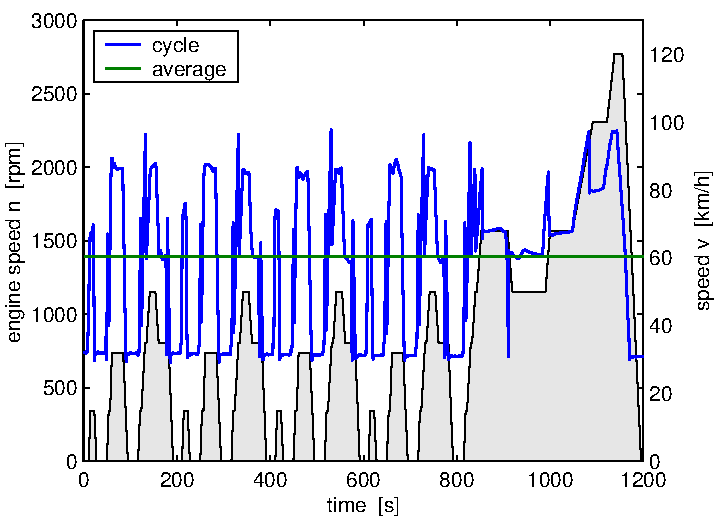
\includegraphics[width = \textwidth]{images/cycle_we.pdf}
  \end{minipage}
  \hfill
  \begin{minipage}[t]{0.48\textwidth}
    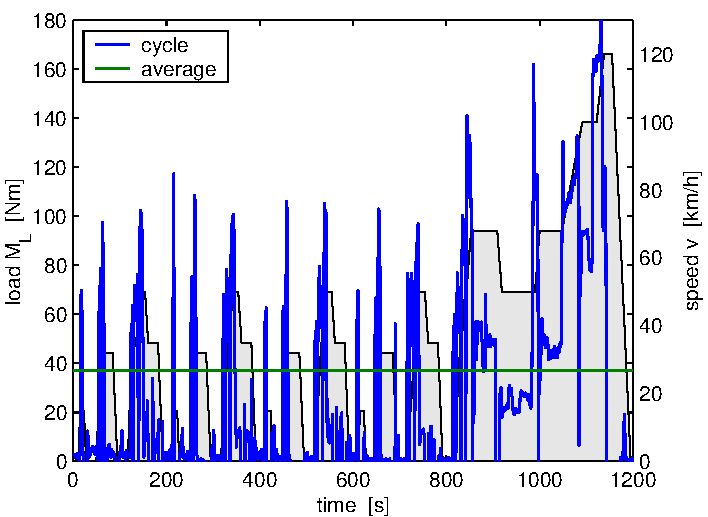
\includegraphics[width = \textwidth]{images/cycle_ml.pdf}
  \end{minipage}
  \caption{Zwei Bilder nebeneinander.}
  \label{pics:cycle}
\end{figure}
\end{verbatim}

\begin{figure}
  \begin{minipage}[t]{0.48\textwidth}
    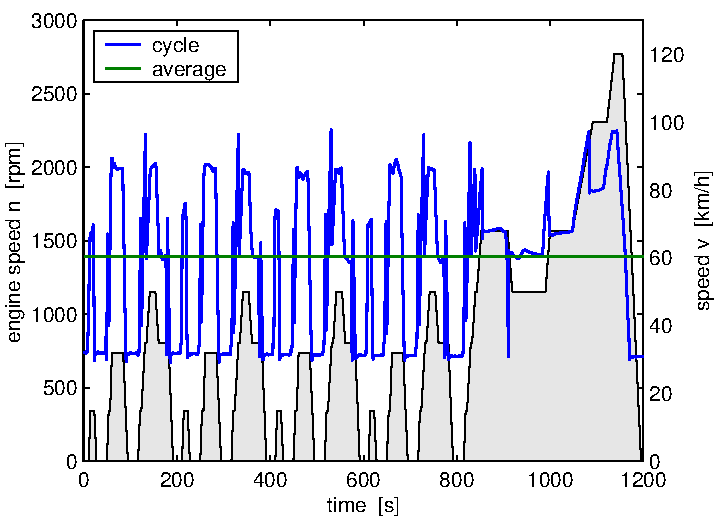
\includegraphics[width = \textwidth]{images/cycle_we.pdf}
  \end{minipage}
  \hfill
  \begin{minipage}[t]{0.48\textwidth}
    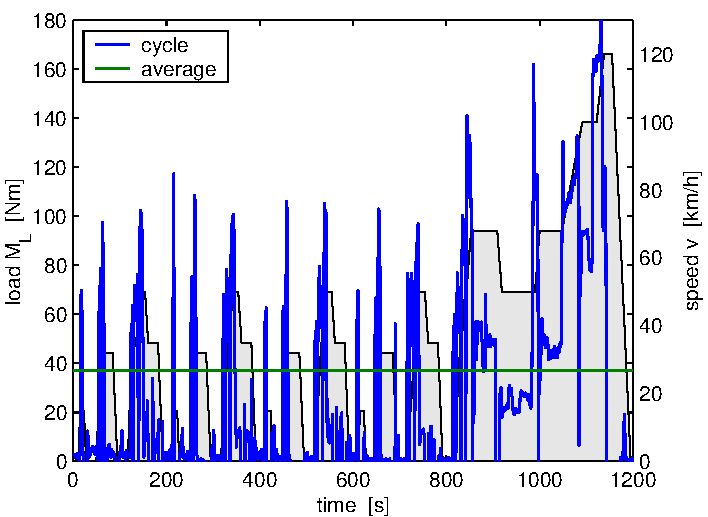
\includegraphics[width = \textwidth]{images/cycle_ml.pdf}
  \end{minipage}
  \caption{Zwei Bilder nebeneinander}
  \label{pics:cycle}
\end{figure}


\section{Mathematische Formeln}\label{sec:math}

Einfache mathematische Formeln werden mit der equation-Umgebung
erzeugt:
\begin{equation}
 p_{me0f}(T_e,\omega_e) \ = \ k_1(T_e) \cdot (k_2+k_3 S^2
 \omega_e^2) \cdot \Pi_{\mathrm{max}} \cdot \sqrt{\frac{k_4}{B}} \, .
 	\label{eq:my_equation}
\end{equation}

Der Code dazu lautet:
\begin{verbatim}
\begin{equation}
 p_{me0f}(T_e,\omega_e) \ = \ k_1(T_e) \cdot (k_2+k_3 S^2
 \omega_e^2) \cdot \Pi_{max} \cdot \sqrt{\frac{k_4}{B}} \, .
\end{equation}
\end{verbatim}

Mathematische Ausdrücke im Text werden mit \$formel\$ erzeugt (z.B.:
$a^2+b^2=c^2$).

Vektoren und Matrizen werden mit den Befehlen \texttt{\textbackslash vec\{.\}} und \texttt{\textbackslash mat\{.\}} erzeugt (z.B. $\vec{v}$, $\mat{M}$).


\section{Weitere nützliche Befehle}\label{sec:div}

Hervorhebungen im Text sehen so aus: \emph{hervorgehoben}. Erzeugt
werden sie mit dem \texttt{\textbackslash epmh\{.\}} Befehl.

Einheiten werden mit den Befehlen \texttt{\textbackslash unit[1]\{m\}} (z.B.~\unit[1]{m}) und \texttt{\textbackslash unitfrac[1]\{m\}\{s\}} (z.B.~\unitfrac[1]{m}{s}) gesetzt.
